\subsubsection{The ``inclusion'' Stokes benchmark}
\label{sec:benchmark-inclusion}

The ``inclusion'' benchmark again solves a problem with a discontinuous
viscosity, but this time the viscosity is chosen in such a way that the
discontinuity is along a circle. This ensures that, unlike in the SolCx
benchmark discussed above, the discontinuity in the viscosity never aligns to
cell boundaries, leading to much larger difficulties in obtaining an accurate
representation of the pressure. Specifically, the almost discontinuous
pressure along this interface leads to oscillations in the numerical
solution. This can be seen in the visualizations shown in
Fig.~\ref{fig:inclusion}. As before, for details we refer to
\cite{DMGT11}. The analytic solution against which we compare is given in
\cite{SP03}. An extensive discussion of convergence properties is given in
\cite{KHB12}.

\begin{figure}
  \begin{center}
    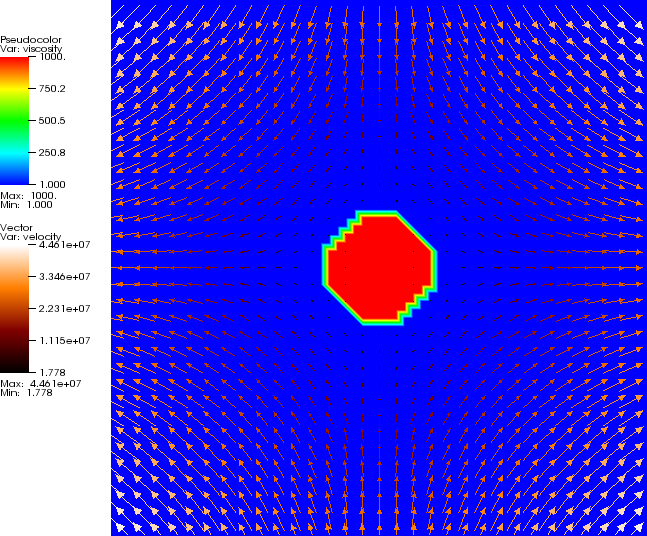
\includegraphics[width=0.45\textwidth]{cookbooks/benchmarks/inclusion/doc/inclusion-solution.png}
    \hfill
    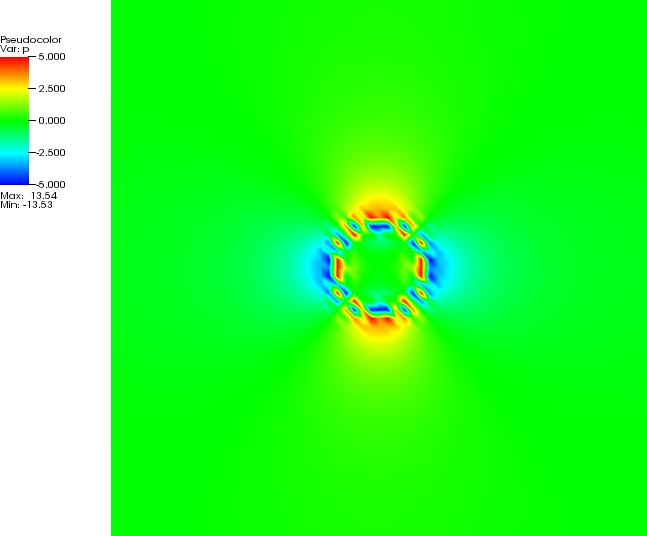
\includegraphics[width=0.45\textwidth]{cookbooks/benchmarks/inclusion/doc/inclusion-solution-pressure.png}
    \caption{\it Inclusion Stokes benchmark. Left: The viscosity field
      when interpolated onto the mesh (internally, the ``exact'' viscosity
      field -- large inside a circle, small outside -- is used),
      and overlaid to it some velocity vectors. Right: The
      pressure with its oscillations along the interface. The oscillations
      become more localized as the mesh is refined.}
    \label{fig:inclusion}
  \end{center}
\end{figure}

The benchmark can be run using the parameter files in \url{benchmarks/inclusion/}. The material model, boundary condition, and postprocessor are defined in \url{benchmarks/inclusion/inclusion.cc}. Consequently, this code needs to be compiled into a shared lib before you can run the tests.

\marginpar{Link to a general section on how you can compile libs for the benchmarks.}

\marginpar{Revisit this once we have the machinery in place to choose nonzero
  boundary conditions in a more elegant way.}

\marginpar{The following prm file isn't annotated yet. How to annotate if we have a .lib?}

\lstinputlisting[language=prmfile]{cookbooks/benchmarks/inclusion/doc/inclusion.prm.out}
